\documentclass[a4paper,debug]{tufte-handout}

\def\TheTitle{Code Loops: There and Back Again}

\title{\TheTitle}
\date{\today}
\author{Ben Nagy and David Michael Roberts}

\setlength{\parindent}{0pt}

\usepackage[lined,boxruled,commentsnumbered]{algorithm2e}

\usepackage{amsmath,amsthm}

\theoremstyle{plain}
\newtheorem{theorem}{Theorem}
\newtheorem{lemma}[theorem]{Lemma}
\newtheorem{proposition}[theorem]{Proposition}
\newtheorem{corollary}[theorem]{Corollary}

\theoremstyle{definition}
\newtheorem{definition}[theorem]{Definition}

\theoremstyle{remark}
\newtheorem{example}[theorem]{Example}
\newtheorem{remark}[theorem]{Remark}

\usepackage{url,graphicx}

\hypersetup{
urlcolor = red,
colorlinks = true,
linkcolor = blue,
citecolor = blue,
linktocpage = true,
pdftitle = {\TheTitle},
pdfauthor = {Ben Nagy, David M. Roberts},
bookmarksopen = false,
bookmarksopenlevel = 1,
unicode = true,
hypertexnames =false
}%

\DeclareMathOperator{\Hamming}{Hamming}
\DeclareMathOperator{\dom}{dom}
\DeclareMathOperator{\Span}{span}
\newcommand{\F}{\mathbb{F}}
\def\cP{\mathcal{P}}
\def\FF{\mathbb{F}}


\begin{document}

\maketitle

\medskip

\subsection{Abstract}
\noindent This paper will describe an implementation of an algorithm by Griess to construct a twisted cocycle describing the multiplication in a code loop, as well as a method to reconstruct the full cocycle from a function defined on a domain of size approximately the square root of the original. 
\marginnote{Every sentence should start on a new line in the source}Additionally, we find a new basis for the extended Golay code with the property that the twisted cocycle built from it by Griess' algorithm is trivial on a pair of subspaces with trivial intersection, of dimensions 6 and 5 respectively.


\section{Intro}

A \emph{loop} is an algebraic structure generalising that of a group, where the axiom of associativity is lost, but the property that left and right multiplication by any fixed element is a bijection is added as a new axiom.
Even nicer than general loops are \emph{Moufang} loops, which satisfy a weak variant of associativity, namely
\[
	z(x(zy)) = ((zx)z)y.
\]
One interesting class of finite Moufang loops are constructed from \emph{doubly-even codes}---certain nice subspaces of vector fields over $\FF_2$)---and so are called \emph{code loops}. 
These were introduced by Griess\cite{Griess} as a general framework to include the Parker loop $\cP$, used by Conway as one ingredient in constructing the Monster group.

Code loops are central extensions, in the category of codes, of the underlying additive group of a doubly-even code $C$:
\[
	1\to \FF_2 \to \widetilde{C} \to C \to 1
\]
Much as central extensions of groups can be described by, and constructed from, 2-cocycles, a central extension as above can be described by a \emph{twisted cocycle} $\theta\colon C\times C \to \FF_2$. 
Instead of the cocycle identity, $\theta$ must satisfy
\[
	\theta(x,y) + \theta(x,y+z) + \theta(x+y,z) + \theta(y,z) = |x\wedge y \wedge z|,
\]
where $\wedge$ is co\"ordinate-wise multiplication,\marginnote{that is, bit-wise AND} and $|\cdot|$ is the bit-weight of a vector, namely the number of non-zero entries.

Griess outlines a method to compute $\theta$, given a total flag in the code $C$, as an existence proof for code loops.
However, it is far from obvious what properties the resulting twisted cocycle (and so the code loop) has, apart from being unique up to a coboundary.
This paper gives an implementation of Griess' procedure and a means of reconstructing any value of a precalculated twisted cocycle from a  lookup table much smaller that the full data of the twisted cocycle.
This will ideally lead to feasable computation with the Parker loop.


\section{The algorithm}

Griess' method starts by choosing a total flag and then choosing a specified new vector in each higher-dimensional subspace, but we have rather chosen to input a basis $\{v_0,\ldots,v_{n-1}\}$, and then generate the flag $V_0 \subset V_1 \subset \cdots \subset V_{n-1} = C$ as $V_i = \Span\{v_0,\ldots,v_i\}$.
Ater an initialisation step (D0), the algorithm loops through steps D1-D4 for each subspace $V_1$,\ldots,$V_{n-1}$.

Here's a sample of the first pass of the algorithm, though we need to check this against the implementation, and it should generalise to $v \in \Span(\text{already considered vectors})$.\sidenote{I guess we should use some kind of algorithm package to write this up? Eg \url{https://en.wikibooks.org/wiki/LaTeX/Algorithms}}

\begin{algorithm}[H]
\SetAlgoLined
\KwData{basis $\{b_0,b_1,\ldots,b_{n-1}\}$ for the code $C$}
\KwResult{twisted cocycle $\theta\colon C\times C\to \FF_2$, encoded as a square array of elements from $\FF_2$, with rows and columns indexed by $C$ }
Initialise: set all values to $0$\;
\tcp{step D0: Vk here is span(b0)}
$\theta(b_0,b_0) \leftarrow |b_0|/4 \mod 2$\;
\ForAll{$1\leq k\leq n-1$}{
	Define $V_k :=\Span\{b_0,\ldots,b_{k-1}\}$\;
	\tcp{step D1: define theta on \{bk\} x Vk and deduce on Vk x \{bk\}}
	\ForAll{$v\in V_k$}{
		\eIf{$v\neq0$}{
			$\theta(b_k,v) \leftarrow \text{random}$\;
			$\theta(v,b_k) \leftarrow |v\wedge b_k|/2+\theta(b_k,v) \mod 2$\;
		}
		{
			\tcp{$\theta(b_k,v)$ is already implicity set to $0$}
			$\theta(v,b_k)\leftarrow |v\wedge b_k| \mod 2$ (but isn't this also always $0$?)\;
		}
	}
	\tcp{step D2: deduce theta on \{bk\} x Wk and Wk x \{bk\}}
	\ForAll{$v\in V_k$}{
		$\theta(b_k,b_k+v) \leftarrow |b_k|/4 + \theta(b_k,v)\mod 2$\;
		$\theta(b_k+v,b_k) \leftarrow |b_k\wedge (b_k+v)|/2 + |b_k|/4 + \theta(b_k,v)\mod 2$\;
	}
	\tcp{step D3: deduce theta on Wk x Wk}
	\ForAll{$v_1\in V_k$}{
		\ForAll{$v_2\in V_k$}{
			$w\leftarrow b_k + v_2$\;
			$a\leftarrow \theta(v_1,b_k)$\;
			$b\leftarrow \theta(v_1,b_k+w)$ (but isn't $b_k+w=v_2$?)\;
			$c\leftarrow \theta(w,b_k)$\;
			$r \leftarrow |v_1\wedge w|/2 + a + b + c \mod 2$\;
			$\theta(w,b_k+v_1) \leftarrow r$
		}
	}
	\tcp{step D4: deduce theta on Wk x Vk and Vk x Wk}
	\ForAll{$v_1\in V_k$}{
		\ForAll{$v_2\in V_k$}{
			$w\leftarrow b_k + v_2$\;
			$a\leftarrow \theta(w,v_1+w)$\;
			$\theta(w,v_1) \leftarrow |w|/4 + a \mod 2$\;
			$\theta(v_1,w) \leftarrow |v\wedge w|/2 + |w|/4 + a \mod 2$\;
		}
	}
}
\caption{Extracted from Griess' proof of existence of twisted cocycles for code loops}
\end{algorithm}

\begin{itemize}

	\item[D0:] $\theta(0,0) = \theta(0,v_0) = \theta(v_0,0) = 0, \quad \theta(v_0,v_0) = |v_0|/4$.

	\item[D1:] For all $x \in \Span\{v_0\}$, 
	\begin{itemize}
		\item[] $\theta(v_1,x) = 0$, \marginnote{arbitrary choice, but with $\theta(v_1,0)=0$}
		\item[] $\theta(x,v_1) = |x\cap v_1|/2$.
	\end{itemize}

	\item[D2:] For all $x \in \Span\{v_0\}$,
	\begin{itemize}
	 	\item[] $\theta(v_1,v_1+x) = |v_1|/4$,
	 	\item[] $\theta(v_1 + x,v_1) = |v_1|/4 + |v_1\cap(v_1+x)|/2$.
	 \end{itemize} 
	 \item[D3:] For all $x,y\in \Span\{v_0\}$,
	 \begin{itemize}
	 	\item[] $\theta(v_1+x,v_1+y) = |y\cap(v_1+x)|/2 + |y\cap v_1|/2 + \theta(x,y) + |v_1|/4 + |v_1\cap(v_1+x)|/2$.
	 \end{itemize}
	 \item[D4:] For all $x,y\in \Span\{v_0\}$,
	 \begin{itemize}
	 	\item[] $\theta(v_1+x,y) = |v_1+x|/4 + \theta(v_1+x,v_1+x+y)$,
	 	\item[] $\theta(y,v_1+x) = |y\cap(v_1+x)|/2 + \theta(v_1+x,y)$.
	 \end{itemize}

\end{itemize} 

\section{Implementation}

All kinds of crazy bit-level tricks...

Benchmarking etc.

\section{Reducing the size of the domain} 
We can split $C$ as $V\oplus W$ and denote the restriction of $\theta$ to $(V\cup W)\times (V \cup W)$ by $\alpha$, that is, a function
\[
	\begin{array}{ccc}
		V\times V& \cup&V\times W\\
		\cup&&\cup\\
		W\times V&\cup &W\times W
	\end{array} \longrightarrow \F_2.
\]

\begin{proposition}\label{eq:reconstructing theta}

We can write $\theta$ entirely in terms of $\alpha$ as follows:
\begin{align*}
	\theta(v_1+w_1,v_2+w_2)	& = \alpha(v_1,v_2)  + \alpha(w_1,w_2) + \alpha(v_1,w_1) + \alpha(w_2,v_2) + \alpha(v_1+v_2,w_1+w_2)\\
							& + \frac12|v_2\wedge(w_1+w_2)| + |v_1\wedge v_2 \wedge (w_1+w_2)| + |w_1\wedge w_2 \wedge v_2| + |v_1\wedge w_1 \wedge (v_2 + w_2)| 
\end{align*}
\end{proposition}

Note that the domain of $\alpha$ has size $(2^k + 2^l - 1)^2$, whereas the domain of $\theta$ has size $2^{2(k+l)}$, where $k=\dim V$ and $l=\dim W$.
If $k=l$, then $|\dom(\alpha)| = (2^{k+1}-1)^2 \approx \sqrt{|\dom(\theta)|} = 2^{4k}$.

So if $\theta$ has been already calculated using the algorithm in the section `Griess' algorithm', then one only needs to store $\alpha$, and use Proposition~\ref{eq:reconstructing theta} to calculate any other values on the fly.

\section{Pretty pictures}

Here is $\alpha$ (badly displayed because of .png$\to$.pdf, but we can make a svg one in Go)

\begin{center}
	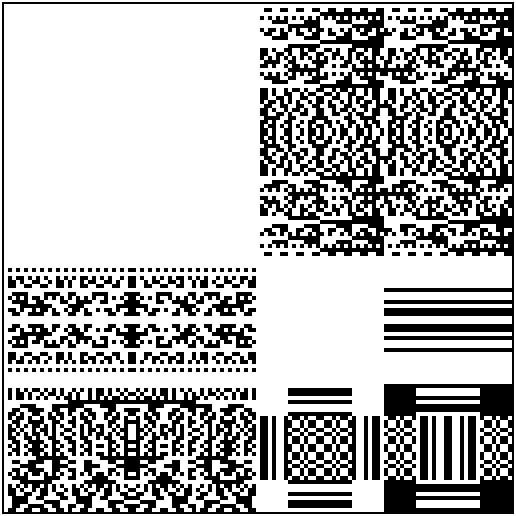
\includegraphics[width=\textwidth]{alpha555_no_label.png}
\end{center}

\bibliographystyle{alpha}
\bibliography{bib}
\end{document}